\documentclass{math}

\usepackage{tikz}

\title{University Physics 2}
\author{Alvin Lin}
\date{January 2018 - May 2018}

\begin{document}

\maketitle

\section*{Electric Flux}
Light, magnetism, heat, and water can all have flux. Flux is defined as the flow
of some field through a surface.
\[ \Phi_{E} = \vec{E}\cdot\vec{A} \]
\[ \vec{A} = A\vec{n} \]
\( \vec{A} \) is an area centered on the surface, with the magnitude equal to
the area and the direction pointing normal to the surface. For a figure with
multiple surfaces:
\[ \Phi_E = \sum\vec{E}\cdot\Delta\vec{A} \]
Gauss's Law states that the electric flux through a closed surface is
proportional to the charge inside the surface (denoted \( Q_{enc} \)).
\[ \Phi_E = \frac{Q_{enc}}{\epsilon_{\circ}} \quad
  K = \frac{1}{4\pi\epsilon_{\circ}} \]
\[ \Phi_E = \oint\vec{E}\cdot\diff{\vec{A}} =
  \frac{Q_{enc}}{\epsilon_{\circ}} \]

\subsection*{Gauss's Law for a Point Charge}
\begin{center}
  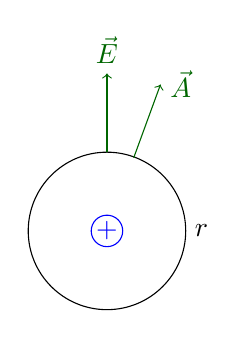
\begin{tikzpicture}
    \draw[blue] (0,0) circle (0.2cm) node {+};
    \draw (0,0) circle (1cm) node[xshift=1.2cm] {\( r \)};
    \draw[->,black!60!green] (0,1) -- (0,2) node[above] {\( \vec{E} \)};
    \draw[->,black!60!green] (0.34,0.93) -- (0.68,1.86)
      node[right] {\( \diff{\vec{A}} \)};
  \end{tikzpicture}
\end{center}
Use Gauss's Law to find \( \vec{E} \) at \( r \) given a point charge surrounded
by a spherical shell of radius \( r \):
\begin{align*}
  \oint\vec{E}\cdot\diff{\vec{A}} &= \frac{Q_{enc}}{\epsilon_{\circ}} \\
  &= \oint|\vec{E}||\diff{\vec{A}}|\cos\theta \\
  \theta &= 0 \text{ via spherical symmetry} \\
  &= \oint|\vec{E}||\diff{\vec{A}}| \\
  &= |\vec{E}|\oint|\diff{\vec{A}}|
    \text{ since } E \text{ is constant over } r \\
  &= |\vec{E}|4\pi r^2 \\
  |\vec{E}|4\pi r^2 &= \frac{Q}{\epsilon_{\circ}} \\
  |\vec{E}| &= \frac{1}{4\pi r^2}\frac{Q}{\epsilon_{\circ}}
    \text{ (Coulomb's Law)}
\end{align*}

\subsection*{Solving Gauss's Law}
\begin{enumerate}
  \item Draw a picture with axes, distances, coordinates, \( \diff{q} \),
  \( \vec{E} \) fields, \( \diff{\vec{A}} \).
  \item Decide how to solve the problem. For 3D symmetric charge distribution,
  use Gauss's Law. For 2D rings or lines, use the integral form of Coulomb's
  Law.
  \item Pick a Gaussian surface. For objects with spherical symmetry, use a
  shell. For objects with cylindrical symmetry, use a hollow cylinder. For
  objects with planar symmetry, use a box or cylinder.
  \item Write Gauss's Law:
  \[ \oint\vec{E}\cdot\diff{\vec{A}} = \frac{Q_{enc}}{\epsilon_{\circ}} \]
  \item Use symmetry to solve the left hand side. Always pick a Gaussian surface
  so that \( \vec{E} \) is parallel to \( \diff{\vec{A}} \) so that
  \( \vec{E}\cdot\diff{\vec{A}} = |\vec{E}||\diff{\vec{A}}| \).
  \item Also argue via symmetry that \( |\vec{E}| \) is independent of
  integrating variables so that \( \int|\vec{E}||\diff{\vec{A}}| =
  |\vec{E}|\oint\diff{\vec{A}} \).
  \item Solve the integral for the area. \( |\vec{E}|\oint\diff{\vec{A}} =
  |\vec{E}|A \). For a shell, \( A = 4\pi r^2 \). For the side of a cylindrical
  surface, \( A = 2\pi rh \). For the top and bottom of a cylindrical surface,
  \( A = \pi r^2 \).
  \item Calculate \( Q_{enc} \), this can be easy or hard depending on the
  problem. Remember that \( Q = \rho V \).
  \item Solve for \( |\vec{E}| \).
\end{enumerate}

\subsection*{Gauss's Law for a Spherical Solid}
\subsubsection*{Case \( r > a \):}
\begin{center}
  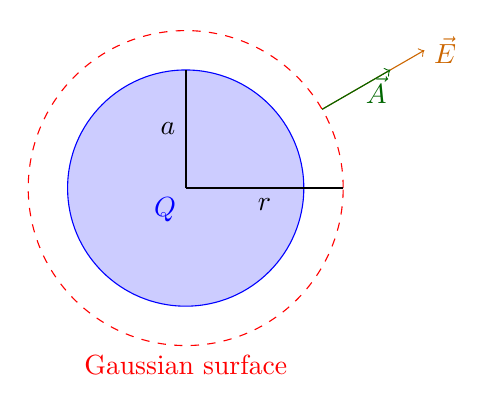
\begin{tikzpicture}
    \draw[blue,fill=white!80!blue] (0,0) circle (1.5cm)
      node[below left] {\( Q \)};
    \draw[red,dashed] (0,0) circle (2cm)
      node[yshift=-2cm, below] {Gaussian surface};
    \draw[thick] (0,0) -- (2,0) node[pos=0.5,below] {\( r \)};
    \draw[thick] (0,0) -- (0,1.5) node[pos=0.5,left] {\( a \)};
    \draw[black!20!orange,->] ({2*cos(30)},{2*sin(30)}) --
      ({3.5*cos(30)},{3.5*sin(30)}) node[right] {\( \vec{E} \)};
    \draw[black!60!green,->] ({2*cos(30)},{2*sin(30)}) --
      ({3*cos(30)},{3*sin(30)}) node[pos=0.5,right] {\( \diff{\vec{A}} \)};
  \end{tikzpicture}
\end{center}
\[ \oint\vec{E}\cdot\diff{\vec{A}} = \int|\vec{E}||\diff{\vec{A}}| =
  |\vec{E}|\int|\diff{\vec{A}}| = |\vec{E}|A = |\vec{E}|4\pi r^2 \]
We can make this argument because \( \vec{E} \) and \( \diff{\vec{A}} \) are
both radial and parallel to each other. The electric field is also constant
over \( r \) by spherical symmetry, so we can bring it outside the integral.
Since we are working with a Gaussian surface whose radius \( r \) is greater
than the radius of the solid \( a \), the enclosed charge is just the total
charge.
\begin{align*}
  |\vec{E}|4\pi r^2 &= \frac{Q_{enc}}{\epsilon_{\circ}} =
    \frac{Q}{\epsilon_{\circ}} \\
  |\vec{E}| &= \frac{1}{4\pi r^2}\frac{Q}{\epsilon_{\circ}} \\
  \vec{E} &= \frac{1}{4\pi r^2}\frac{Q}{\epsilon_{\circ}}\hat{r} \\
\end{align*}
Note that the formula for the electric field in this case is just like that of
a point charge.

\subsubsection*{Case \( r < a \):}
\begin{center}
  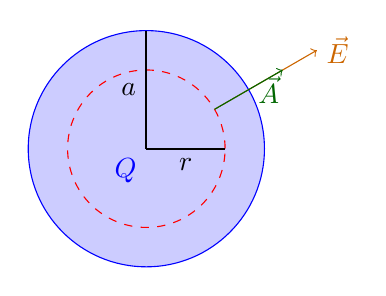
\begin{tikzpicture}
    \draw[blue,fill=white!80!blue] (0,0) circle (1.5cm)
      node[below left] {\( Q \)};
    \draw[red,dashed] (0,0) circle (1cm);
    \draw[thick] (0,0) -- (1,0) node[pos=0.5,below] {\( r \)};
    \draw[thick] (0,0) -- (0,1.5) node[pos=0.5,left] {\( a \)};
    \draw[black!20!orange,->] ({cos(30)},{sin(30)}) --
      ({2.5*cos(30)},{2.5*sin(30)}) node[right] {\( \vec{E} \)};
    \draw[black!60!green,->] ({cos(30)},{sin(30)}) --
      ({2*cos(30)},{2*sin(30)}) node[pos=0.5,right] {\( \diff{\vec{A}} \)};
  \end{tikzpicture}
\end{center}
\[ \oint\vec{E}\cdot\diff{\vec{A}} = |\vec{E}|4\pi r^2 \]
This argument can be made for the same reasons as above. The enclosed charge
must be expressed in terms of \( r \) now. For this problem, we can assume the
charge is uniform, which means it can be expressed using the following ratio:
\begin{align*}
  \rho &= \frac{Q_{total}}{V_{total}} = \frac{Q_{enc}}{V_{enc}} \\
  Q_{enc} &= \frac{Q_{total}V_{enc}}{V_{total}} \\
  &= \frac{Q}{\frac{4}{3}\pi a^3}\frac{4}{3}\pi r^3 \\
  &= \frac{Qr^3}{a^3}
\end{align*}
Now we can solve for \( |\vec{E}| \):
\begin{align*}
  |\vec{E}|4\pi r^2 &= \frac{Q_{enc}}{\epsilon_{\circ}} =
    \frac{Qr^3}{\epsilon_{\circ}a^3} \\
  |\vec{E}| &= \frac{1}{4\pi r^2}\frac{Qr^3}{\epsilon_{\circ}a^3}
    = \frac{1}{4\pi}\frac{Qr}{\epsilon_{\circ}a^3} \\
\end{align*}
From these two results, we can see that the electric field increases linearly
inside the solid up to \( a \), and then decreases proportionally to
\( \frac{1}{r^2} \).

\subsection*{Gauss's Law for a Spherical Hollow Shell}
\subsubsection*{Case \( r < a \):}
\begin{center}
  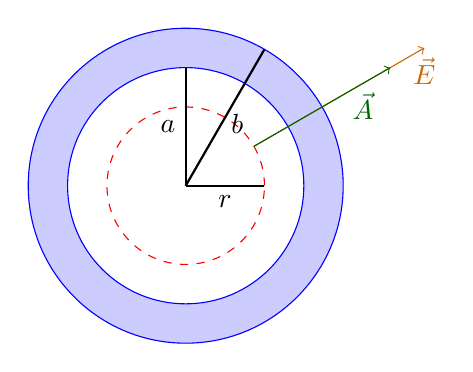
\begin{tikzpicture}
    \fill[white!80!blue] (2,0) arc (360:0:2cm) -- (1.5,0) arc (0:360:1.5cm);
    \draw[blue] (0,0) circle (2cm);
    \draw[blue] (0,0) circle (1.5cm);
    \draw[red,dashed] (0,0) circle (1cm);
    \draw[thick] (0,0) -- (1,0) node[pos=0.5,below] {\( r \)};
    \draw[thick] (0,0) -- (0,1.5) node[pos=0.5,left] {\( a \)};
    \draw[thick] (0,0) -- ({2*cos(60)},{2*sin(60)})
      node[pos=0.45,right] {\( b \)};
    \draw[black!20!orange,->] ({cos(30)},{sin(30)}) --
      ({3.5*cos(30)},{3.5*sin(30)}) node[below] {\( \vec{E} \)};
    \draw[black!60!green,->] ({cos(30)},{sin(30)}) --
      ({3*cos(30)},{3*sin(30)})
      node[pos=0.8,below] {\( \diff{\vec{A}} \)};
  \end{tikzpicture}
\end{center}
\[ \oint\vec{E}\cdot\diff{\vec{A}} = |\vec{E}|4\pi r^2 \]
The same argument as above can be applied here. Since the Gaussian surface is
inside the solid, it encloses no charge, meaning \( Q_{enc} = 0 \).
\begin{align*}
  |\vec{E}|4\pi r^2 &= \frac{Q_{enc}}{\epsilon_{\circ}} = 0 \\
  |\vec{E}| &= 0 \\
  \vec{E} &= \vec{0}
\end{align*}
The electric field anywhere inside the solid is zero.

\subsubsection*{Case \( a < r < b \):}
\begin{center}
  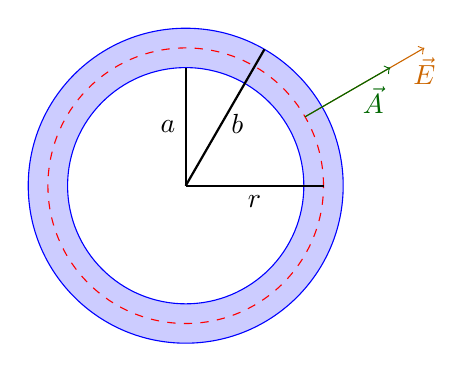
\begin{tikzpicture}
    \fill[white!80!blue] (2,0) arc (360:0:2cm) -- (1.5,0) arc (0:360:1.5cm);
    \draw[blue] (0,0) circle (2cm);
    \draw[blue] (0,0) circle (1.5cm);
    \draw[red,dashed] (0,0) circle (1.75cm);
    \draw[thick] (0,0) -- (1.75,0) node[pos=0.5,below] {\( r \)};
    \draw[thick] (0,0) -- (0,1.5) node[pos=0.5,left] {\( a \)};
    \draw[thick] (0,0) -- ({2*cos(60)},{2*sin(60)})
      node[pos=0.45,right] {\( b \)};
    \draw[black!20!orange,->] ({1.75*cos(30)},{1.75*sin(30)}) --
      ({3.5*cos(30)},{3.5*sin(30)}) node[below] {\( \vec{E} \)};
    \draw[black!60!green,->] ({1.75*cos(30)},{1.75*sin(30)}) --
      ({3*cos(30)},{3*sin(30)})
      node[pos=0.8,below] {\( \diff{\vec{A}} \)};
  \end{tikzpicture}
\end{center}
\[ \oint\vec{E}\cdot\diff{\vec{A}} = |\vec{E}|4\pi r^2 \]
The same argument as above can be applied here. The enclosed charge must be
expressed in terms of \( r \) now.
\[ Q_{enc} = \int\rho\diff{V} = \rho V =
  \rho(\frac{4}{3}\pi r^3-\frac{4}{3}\pi a^3) = \frac{4}{3}\pi\rho(r^3-a^3) \]
Now we can plug this back into Gauss's Law:
\begin{align*}
  |\vec{E}|4\pi r^2 &= \frac{Q_{enc}}{\epsilon_{\circ}} =
    \frac{1}{\epsilon_{\circ}}\frac{4}{3}\pi\rho(r^3-a^3) \\
  |\vec{E}| &= \frac{1}{4\pi r^2\epsilon_{\circ}}\frac{4}{3}\pi\rho(r^3-a^3) \\
  &= \frac{\rho}{3\epsilon_{\circ}}\frac{r^3-a^3}{r^2}
\end{align*}
Note that inside the solid, the charge increases linearly.

\subsubsection*{Case \( r > b \):}
\begin{center}
  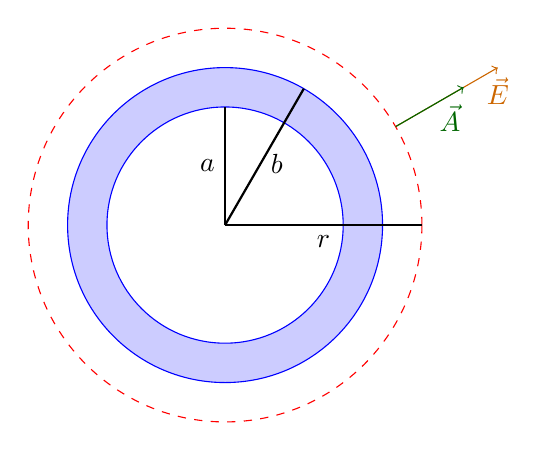
\begin{tikzpicture}
    \fill[white!80!blue] (2,0) arc (360:0:2cm) -- (1.5,0) arc (0:360:1.5cm);
    \draw[blue] (0,0) circle (2cm);
    \draw[blue] (0,0) circle (1.5cm);
    \draw[red,dashed] (0,0) circle (2.5cm);
    \draw[thick] (0,0) -- (2.5,0) node[pos=0.5,below] {\( r \)};
    \draw[thick] (0,0) -- (0,1.5) node[pos=0.5,left] {\( a \)};
    \draw[thick] (0,0) -- ({2*cos(60)},{2*sin(60)})
      node[pos=0.45,right] {\( b \)};
    \draw[black!20!orange,->] ({2.5*cos(30)},{2.5*sin(30)}) --
      ({4*cos(30)},{4*sin(30)}) node[below] {\( \vec{E} \)};
    \draw[black!60!green,->] ({2.5*cos(30)},{2.5*sin(30)}) --
      ({3.5*cos(30)},{3.5*sin(30)})
      node[pos=0.8,below] {\( \diff{\vec{A}} \)};
  \end{tikzpicture}
\end{center}
\[ \oint\vec{E}\cdot\diff{\vec{A}} = |\vec{E}|4\pi r^2 \]
This same argument as above can be applied here. Like the spherical solid, since
the Gaussian surface is larger than the solid, the enclosed charge is just the
total charge.
\begin{align*}
  |\vec{E}|4\pi r^2 &= \frac{Q_{enc}}{\epsilon_{\circ}} =
    \frac{Q}{\epsilon_{\circ}} \\
  |\vec{E}| &= \frac{1}{4\pi r^2}\frac{Q}{\epsilon_{\circ}} \\
  \vec{E} &= \frac{1}{4\pi r^2}\frac{Q}{\epsilon_{\circ}}\hat{r} \\
\end{align*}
Notice that this formula is again very much like that of a point charge. For
this spherical hollow, it can also be written as:
\[ |\vec{E}| = \frac{\rho}{3\epsilon_{\circ}}\frac{b^3-a^3}{r^2} \]

\section*{Important Relations}
\begin{align*}
  \lambda &= \frac{Q}{L} \\
  \sigma &= \frac{Q}{A} \\
  \rho &= \frac{Q}{V} = \frac{Q}{AL} = \frac{\lambda}{A} = \frac{\sigma}{L} \\
  Q_{total} &= \int\rho\diff{V}
\end{align*}

\begin{center}
  You can find all my notes at \url{http://omgimanerd.tech/notes}. If you have
  any questions, comments, or concerns, please contact me at
  alvin@omgimanerd.tech
\end{center}

\end{document}
